\documentclass[12pt,a4paper]{article}
\usepackage[utf8]{vietnam}
\usepackage{amsmath,amssymb}
\usepackage{tabularx}
\usepackage{tikz}
\usetikzlibrary{calc,angles,quotes,arrows.meta,patterns}
\usepackage{xcolor}
\usepackage{enumitem}
\usepackage{fancyhdr}
\usepackage{graphicx}
\usepackage[top=0.9cm, bottom=0.9cm, left=1.2cm, right=1.2cm]{geometry}
\usepackage[dethi]{ex_test}
\SAOPTN{widthSA=3.2,heightSA=0.62}

\setlength{\headheight}{15pt}
\setlength{\parskip}{0pt}

\pagestyle{fancy}
\fancyhf{}
\rhead{\textit{Môn Toán 9 -- Đề số 09}}
\lhead{\textit{Bộ đề ôn tập Giữa học kì I}}
\cfoot{\thepage}

\begin{document}

% --- KHUNG TIÊU ĐỀ ĐỀ THI ---
\noindent
\begin{tabularx}{\linewidth}{X r}
\textbf{TRƯỜNG THCS: \dotfill} & \textbf{ĐỀ KIỂM TRA ĐỊNH KỲ GIỮA HỌC KỲ I} \\
\textbf{Họ và tên: \dotfill} & \textbf{NĂM HỌC 2026 -- 2027} \\
\textbf{Lớp: \dotfill \quad SBD: \dotfill} & \textbf{Môn: TOÁN 9} \\
\hline
\end{tabularx}
\vspace{2mm}

\begin{center}
  \textbf{\large ĐỀ ÔN TẬP GIỮA HỌC KỲ I -- ĐỀ SỐ 09}\\
  \textit{Thời gian làm bài: 90 phút (Không kể thời gian phát đề)}
\end{center}
\vspace{1mm}

% --- PHẦN I ---
\noindent\textbf{\large PHẦN I. CÂU TRẮC NGHIỆM NHIỀU PHƯƠNG ÁN LỰA CHỌN (3,0 điểm)}

\textit{Thí sinh trả lời từ câu 1 đến câu 12. Mỗi câu hỏi thí sinh chỉ chọn một phương án duy nhất.}

\vspace{1mm}
\begin{ex}
Phương trình nào sau đây là phương trình bậc nhất hai ẩn?
\choice
{$2x - 4 = 0$}
{$5y - 1 = 3(y - 4)$}
{\True $2x + 7y = 5$}
{$2x^2 + 8y = 0$}
\end{ex}

\begin{ex}
Cặp số $(2; 0)$ là nghiệm của hệ phương trình nào sau đây?
\choice
{$\begin{cases} 2x - 2y = 2 \\ x + 2y = 4 \end{cases}$}
{$\begin{cases} 2x - y = -1 \\ 3x - y = 8 \end{cases}$}
{$\begin{cases} 2x - y = -1 \\ 3x - y = 7 \end{cases}$}
{\True $\begin{cases} 4x - 2y = 8 \\ 3x - 5y = 6 \end{cases}$}
\end{ex}

\begin{ex}
Hệ phương trình nào sau đây là hệ hai phương trình bậc nhất hai ẩn?
\choice
{$\begin{cases} 2x - y = 3 \\ 2x^2 + 3y = 4 \end{cases}$}
{\True $\begin{cases} 3x - y = -1 \\ 5x - 3y = 8 \end{cases}$}
{$\begin{cases} 3x - 2y = 1 \\ \frac{1}{x} - 3y = 7 \end{cases}$}
{$\begin{cases} 2x - y^2 = 4 \\ 2x - 3y = 5 \end{cases}$}
\end{ex}

\begin{ex}
Khẳng định nào sau đây là đúng với mọi $A \ge 0, B \ge 0$?
\choice
{$\sqrt{A \cdot B} = \sqrt{A} \cdot \sqrt{B}$ ($A \ge 0, B > 0$)}
{\True $\sqrt{A \cdot B} = \sqrt{A} \cdot \sqrt{B}$ ($A \ge 0, B \ge 0$)}
{$\sqrt{A \cdot B} = \sqrt{A} \cdot \sqrt{B}$ ($AB \ge 0$)}
{$\sqrt{A \cdot B} = \sqrt{A} \cdot \sqrt{B}$ ($A > 0, B > 0$)}
\end{ex}

\begin{ex}
Với $a < 3$, kết quả rút gọn của biểu thức $\sqrt{(a - 3)^2} - 2(a + 1)$ là:
\choice
{\True $1 - 3a$}
{$-a - 1$}
{$-a - 5$}
{$5 - 3a$}
\end{ex}

\begin{ex}
Kết quả của phép tính $\sqrt{\frac{49}{169} \cdot 0{,}36}$ là:
\choice
{\True $\frac{21}{65}$}
{$\frac{35}{33}$}
{$\frac{42}{13}$}
{$\frac{42}{169}$}
\end{ex}

\begin{ex}
Cho $a > b$, kết luận nào sau đây không đúng?
\choice
{$-a < -b$}
{$-2a < -2b$}
{$a - b > 0$}
{\True $a^2 > b^2$}
\end{ex}

\begin{ex}
Cho tam giác $MNP$ vuông tại $M$ có đường cao $MH$ và góc $\widehat{N} = \alpha$. Tỉ số lượng giác $\cos \alpha$ bằng:
\choice
{\True $\frac{NH}{MN}$}
{$\frac{MP}{MH}$}
{$\frac{MP}{MN}$}
{$\frac{MH}{NM}$}
\end{ex}

\begin{ex}
Trong hình vẽ, bạn Minh đứng ở vị trí $M$, bạn Nam đứng ở vị trí $N$ cùng ở một bên lề đường và cây xanh $C$ nằm đối diện vị trí Nam đứng ở phía bên kia đường. Biết $MN = 3{,}9\text{ m}$ và góc $\widehat{NMC} = 72^\circ$. Tính khoảng cách từ Minh đến cây xanh $C$ (làm tròn kết quả đến hàng đơn vị):
\begin{center}
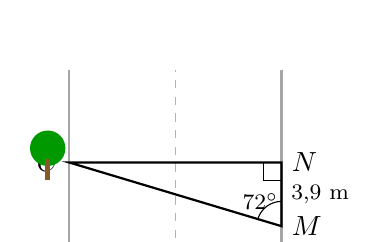
\begin{tikzpicture}[scale=0.9]
  \draw[thick, gray!70] (-1.5,-1.3) -- (-1.5,1.3);
  \draw[thick, gray!70] (1.5,-1.3) -- (1.5,1.3);
  \draw[dashed, gray!60] (0,-1.3) -- (0,1.3);
  \coordinate (C) at (-1.5,0);
  \coordinate (N) at (1.5,0);
  \coordinate (M) at (1.5,-0.9);
  \draw[thick] (C) node[left]{$C$} -- (N) node[right]{$N$} -- (M) node[right]{$M$} -- cycle;
  \draw (N) ++(-0.25,0) -- ++(0,-0.25) -- ++(0.25,0);
  \draw (M) ++(0,0.35) arc (90:162:0.35);
  \node at (1.2,-0.55) {\footnotesize $72^\circ$};
  \node[right] at (1.5,-0.45) {\footnotesize $3{,}9\text{ m}$};
  \fill[green!60!black] (-1.8,0.2) circle (0.25);
  \draw[line width=1.8pt, brown!70!black] (-1.8,0.05) -- (-1.8,-0.25);
\end{tikzpicture}
\end{center}
\choice
{$12\text{ m}$}
{\True $13\text{ m}$}
{$12{,}7\text{ m}$}
{$12{,}6\text{ m}$}
\end{ex}

\begin{ex}
Cho $a > b$, khi đó ta có khẳng định nào đúng?
\choice
{$2a < 2b$}
{$-2a > -2b$}
{\True $2a - 3 > 2b - 3$}
{$-3a - 5 > -3b - 5$}
\end{ex}

\begin{ex}
Cho bất đẳng thức $2a + b \ge 3a$. Vế trái của bất đẳng thức là:
\choice
{$3a$}
{$b$}
{$2a$}
{\True $2a + b$}
\end{ex}

\begin{ex}
Cho tam giác $ABC$ vuông tại $A$. Tỉ số $\sin B$ bằng:
\choice
{$\frac{AB}{BC}$}
{\True $\frac{AC}{BC}$}
{$\frac{AB}{AC}$}
{$\frac{AC}{AB}$}
\end{ex}


\vspace{1mm}
\noindent\textbf{BẢNG TRẢ LỜI TRẮC NGHIỆM PHẦN I:}
\begin{center}
\begin{tabular}{|c|c|c|c|c|c|c|c|c|c|c|c|c|}
\hline
\textbf{Câu} & \textbf{1} & \textbf{2} & \textbf{3} & \textbf{4} & \textbf{5} & \textbf{6} & \textbf{7} & \textbf{8} & \textbf{9} & \textbf{10} & \textbf{11} & \textbf{12} \\
\hline
\textbf{Chọn} & \rule{0pt}{0.65cm} & & & & & & & & & & & \\
\hline
\end{tabular}
\end{center}
\vspace{2mm}

% --- PHẦN II ---
\noindent\textbf{\large PHẦN II. CÂU TRẮC NGHIỆM ĐÚNG SAI (2,0 điểm)}

\textit{Thí sinh trả lời từ câu 1 đến câu 2. Trong mỗi ý a), b), c), d) ở mỗi câu, thí sinh chọn đúng hoặc sai.}

\vspace{1mm}
\begin{ex}
Cho hệ phương trình $\begin{cases} 2x + y = 4 \\ x - y = 2. \end{cases}$ Xét tính Đúng/Sai của các khẳng định sau:
\choiceTF
{\True Cặp số $(2; 0)$ là nghiệm của phương trình thứ nhất.}
{\True Cộng từng vế hai phương trình của hệ ta được phương trình $3x = 6$.}
{\True Nghiệm của hệ phương trình là $(2; 0)$.}
{\True Giá trị biểu thức $M = x^2 - y^2$ tại nghiệm của hệ bằng $4$.}
\end{ex}

\begin{ex}
Cho tam giác $ABC$ vuông tại $A$, đường cao $AH$. Biết $BH = 2\text{ cm}$ và $CH = 8\text{ cm}$. Xét tính Đúng/Sai của các khẳng định sau:
\choiceTF
{\True Độ dài đường cao $AH = 4\text{ cm}$.}
{\True Độ dài cạnh huyền $BC = 10\text{ cm}$.}
{\True Độ dài cạnh $AB = \sqrt{20}\text{ cm}$.}
{\True Giá trị của $\sin B = \frac{2}{\sqrt{5}}$.}
\end{ex}


\vspace{1mm}
\noindent\textbf{BẢNG TRẢ LỜI ĐÚNG SAI PHẦN II:}
\begin{center}
\begin{tabular}{|c|c|c|c|c||c|c|c|c|c|}
\hline
\textbf{Câu} & \textbf{Lệnh hỏi} & \textbf{Đúng} & \textbf{Sai} & \textbf{Điểm} & \textbf{Câu} & \textbf{Lệnh hỏi} & \textbf{Đúng} & \textbf{Sai} & \textbf{Điểm} \\
\hline
 & a) & & & & & a) & & & \\
\cline{2-4}\cline{7-9}
\textbf{1} & b) & & & & \textbf{2} & b) & & & \\
\cline{2-4}\cline{7-9}
 & c) & & & & & c) & & & \\
\cline{2-4}\cline{7-9}
 & d) & & & & & d) & & & \\
\hline
\end{tabular}
\end{center}
\vspace{2mm}

% --- PHẦN III ---
\noindent\textbf{\large PHẦN III. CÂU TRẮC NGHIỆM TRẢ LỜI NGẮN (1,0 điểm)}

\textit{Thí sinh trả lời từ câu 1 đến câu 2. Viết câu trả lời vào ô quy định.}

\vspace{1mm}
\begin{ex}
Giải hệ phương trình $\begin{cases} 3x - 2y = 4 \\ x + 2y = 4. \end{cases}$ Tìm nghiệm $(x; y)$.
\shortans{$(2; 1)$}
\end{ex}

\begin{ex}
Cho tam giác $ABC$ vuông tại $A$, đường cao $AH$. Biết $AB = 6\text{ cm}$ và $AC = 8\text{ cm}$. Tính độ dài đường cao $AH$.
\shortans{$4{,}8\text{ cm}$}
\end{ex}


\vspace{2mm}
% --- PHẦN IV ---
\noindent\textbf{\large PHẦN IV. TỰ LUẬN (4,0 điểm)}

\textit{Thí sinh trình bày chi tiết lời giải vào giấy làm bài.}

\vspace{1mm}
\noindent\textbf{Câu 1 (1,5 điểm).}

Giải các hệ phương trình sau:\par a) $\begin{cases} x + 3y = 2 \\ x + 2y = 5 \end{cases}$\par b) $\begin{cases} 4x - 3y = -1 \\ 2x + 3y = 13. \end{cases}$

\vspace{2mm}
\noindent\textbf{Câu 2 (1,0 điểm).}

Trong kỳ thi tuyển sinh vào lớp 10 Trung học phổ thông, tổng số học sinh dự thi của hai trường THCS $A$ và $B$ là 180 em, tổng số học sinh trúng tuyển là 157 em. Tính số học sinh dự thi và số học sinh trúng tuyển của từng trường, biết trường $A$ có $90\%$ học sinh dự thi trúng tuyển và trường $B$ có $85\%$ học sinh dự thi trúng tuyển.

\vspace{2mm}
\noindent\textbf{Câu 3 (1,0 điểm).}

a) Cho tam giác $DEF$ vuông tại $D$ có $DE = 9\text{ cm}, \widehat{F} = 35^\circ$. Hãy giải tam giác vuông $DEF$ (độ dài các cạnh làm tròn đến hàng phần trăm).\par b) Hai chiếc thuyền $A$ và $B$ ở vị trí được minh họa như hình vẽ. Tính khoảng cách giữa chúng (làm tròn đến hàng phần mười của mét). Biết độ dài $IK = 500\text{ m}, \widehat{AKI} = 50^\circ, \widehat{AKB} = 15^\circ$.
\begin{center}
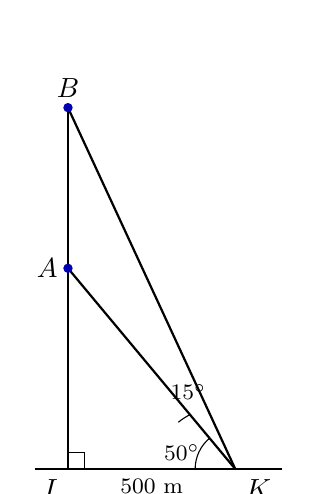
\begin{tikzpicture}[scale=0.85]
  \coordinate (I) at (0,0);
  \coordinate (K) at (2.5,0);
  \coordinate (A) at (0,3.0);
  \coordinate (B) at (0,5.4);
  \draw[thick] (-0.5,0) -- (3.2,0);
  \draw[thick] (I) node[below left]{$I$} -- (K) node[below right]{$K$};
  \draw[thick] (I) -- (B) node[above]{$B$};
  \draw[thick] (K) -- (A) node[left]{$A$};
  \draw[thick] (K) -- (B);
  \draw (I) ++(0,0.25) -- ++(0.25,0) -- ++(0,-0.25);
  \draw (K) ++(-0.6,0) arc (180:130:0.6);
  \node at (1.7,0.25) {\footnotesize $50^\circ$};
  \draw (K) ++(-0.85,0.7) arc (130:115:0.85);
  \node at (1.8,1.15) {\footnotesize $15^\circ$};
  \node[below] at (1.25,0) {\footnotesize $500\text{ m}$};
  \fill[blue!70!black] (A) circle (2pt);
  \fill[blue!70!black] (B) circle (2pt);
\end{tikzpicture}
\end{center}

\vspace{2mm}
\noindent\textbf{Câu 4 (0,5 điểm).}

Cho các số thực $x, y$ thỏa mãn $x^2 + y^2 - 4x + 2y + 5 = 0$. Tính giá trị của biểu thức $P = (x - 3)^{2026} + (y + 2)^{2026}$.

\vspace{2mm}

\vfill
\begin{center}
  \textbf{--- HẾT ---}
\end{center}
\end{document}
